  \chapter{Modelo matemático}\label{cap:modelomat}
  
A idéia utilizada nesssa formulação é que não há necessidade de
modelar os 4 tipos de arcos para cada voo. Para dois voos quaisquer existem
apenas 2 tipos de arcos que podem vir ocorrer como ilustrado na Figura
\ref{fig:modelagem_arcos}.

Em a) os voos respeitam a restrição geográfica, dessa forma apenas os arcos de
tipo 1 e 2 precisam ser modelados uma vez que não teria sentido fazer um voo de
reposicionamento nessa situação. Em b) os aeroportos em questão são diferentes,
sendo necessário apenas a modelagem dos arcos do tipo 3 e 4, perceba que não
teria outra saída se não efetuar um voo de reposicionamento.

\begin{figure}[ht]
	\centering
	\caption{Arcos necessários para ligar dois voos. \mbox{Fonte:
	(Própria)}}\label{fig:modelagem_arcos}
	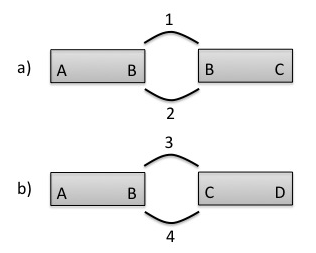
\includegraphics[scale=0.4]{./img/modelagem_arcos}
\end{figure}

Seja $D = (V,A)$ um grafo representando uma instância do PCTA, onde o conjunto de vértice $V = {v_{i}:i \in I}$ de D é indexado por $I = {1, 2, ..., n+1, n+2}$ onde $v_{n+1}$ e $v_{n+2}$, identificam, respectivamente, os nós fonte e destino. E os nós restantes referem-se ao conjunto de arcos originais, com $n$ elementos. Seja os custos ${c_{ij}:(i,j) \in A}$ introduzidos acima, estando associados com cada arco da instância.
  
Seja ${x_{ij}:(i,j) \in A}$ um conjunto binário 0-1 de variáveis usada para controlar a inclusão $(x_{ij} = 1)$ ou a exclusão $(x_{ij} = 0)$ de um arco (possível conexão) entre vértices (voos) $v_{i}$ e $v_{j}$. O conjunto $\overline{I}$ identifica o conjunto de nós excluindo o nó fonte $(v_{n+1})$ e o nó de destino $(v_{n+2})$. Variáveis reais $\delta_{i}$ e $\theta_{i}$, $i \in \overline{I}$ são usados para representar, respectivamente, o desvio do tempo de partida sugerido e a norma desse desvio para $v_{i}$. Essas variáveis devem no entanto obedecer $-\gamma_{i} \geq \delta_{i} \geq \gamma_{i}$ e $0 \geq \theta_{i} \geq \gamma_{i}$, onde $\gamma_{i}$ é o valor máximo de desvio permitido (em cada direção) do tempo de partida sugerido para o voo. Finalmente o tempo de partida sugerido que é dado por $s_{i}:i \in \overline{I}$.
  
\section{Função objetivo}

\begin{equation}
Minimizar \   \ \sum_{i \in I} \sum_{j \in I} x_{ij}c_{ij} + \sum_{i \in \overline{I}} \theta_{i}
\end{equation}

\section{Restrições}

\begin{enumerate}


\item[a)] Garantia de recobrimento dos voos \\
\begin{equation}
  \sum_{i \in I} x_{ij}= 1 \   \ \forall_{j} \in \overline{I} 
\end{equation}
\begin{equation}
\sum_{j \in I} x_{ij} = 1 \   \ \forall_{i} \in \overline{I}
\end{equation}





\item[b)] Viabilidade das conexões \\
\begin{equation}
s_{i} + t_{i}x_{ij} - INF(1 - x_{ij}) + \delta_{i} \leq s_{j} + \delta_{j} \   \ \forall_{i,j} \in \overline{I}
\end{equation}
%\begin{equation}
%\sum_{i \in I} x_{i(n+1)} = 0
%\end{equation}
%\begin{equation}
%\sum_{j \in I} x_{(n+2)j} = 0
%\end{equation}

\item[c)] Modulo do desvio do tempo de partida sugerido \\
\begin{equation}
\theta_{i} \geq \delta_{i} \   \ \forall_{i} \in \overline{I}
\end{equation}
\begin{equation}
\theta_{i} \geq -\delta_{i} \   \ \forall_{i} \in \overline{I}
\end{equation}

\item[d)] Limites das variáveis \\
\begin{equation}
-\gamma_{i} \geq \delta_{i} \geq \gamma_{i} \   \ \forall_{i} \in \overline{I}
\end{equation}
\begin{equation}
0 \geq \theta_{i} \geq \gamma_{i} \   \ \forall{i} \in \overline{I}
\end{equation}
\end{enumerate}

\clearpage

Pode-se perceber que o modelo matemático não faz menção ao tempo de solo ($g$), isso ocorre porque esse tempo é incorporado ao voo como demonstrado na Figura \ref{fig:conversion}, ou seja o tempo de partida sugerido $s$ passa a ter o valor $s - g$ e a duração $t$ do voo passa a ter o valor $t + g$. Uma vantagem de usar essa abordagem que integra o tempo de solo ao voo é que a quantidade de restrições é reduzida.

\begin{figure}[ht]
	\centering
	\caption{Conversão de um voo para ser utilizado no
	solver. \mbox{Fonte: (Própria)}}\label{fig:conversion}
	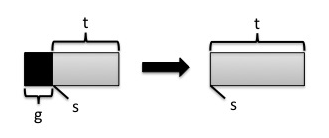
\includegraphics[scale=0.4]{./img/conversion}
	
\end{figure}

Além disso o conjunto $A$ contém apenas um tipo de arco, o arco do tipo 1 se os voos satisfazem a restrição geográfica e o arco do tipo 3 caso não satisfaçam. Os arcos do tipo 2 e 4 são modelados a partir  da variável $\delta$ que tem seu custo acrescentado na função objetivo.

Essa estratégia permite a redução de 3 arcos para cada voo, o que deixa o modelo mais leve.

O calculo dos custos são feitos através de um pré-processamento, onde os arcos viáveis recebem os valores referentes ao seu tipo, por exemplo, no caso de um arco originário do nó source, arco do tipo 6, um custo 1000 é atribuído. No caso de arcos que deverão ser evitados um custo elevado é atribuído.
  	